% !TEX root = paper.tex

\section {Results}
\label{sec:results}

\subsection{Ridge yield}

\begin{figure}[h!]
	\centering
	\subfigure{ 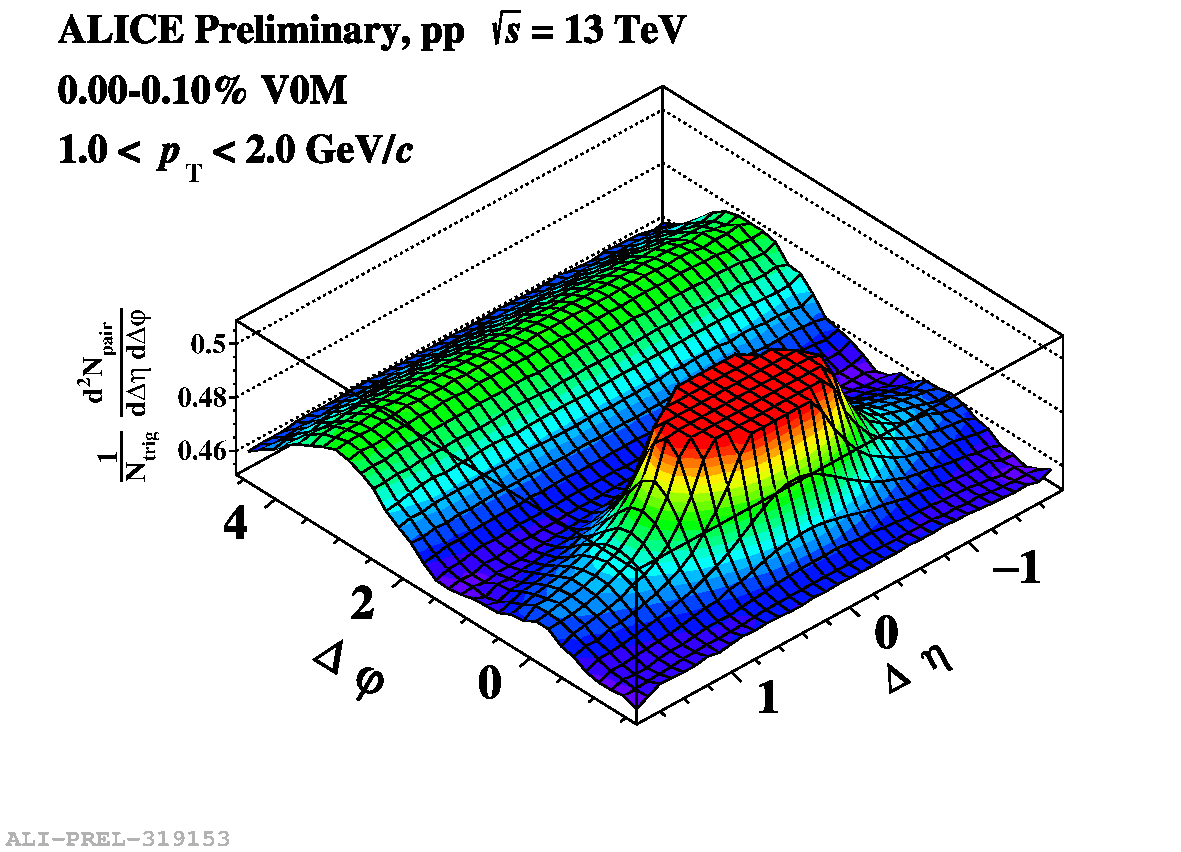
\includegraphics[width=0.47 \textwidth]{./figures/corr1.pdf} }
	\subfigure{ 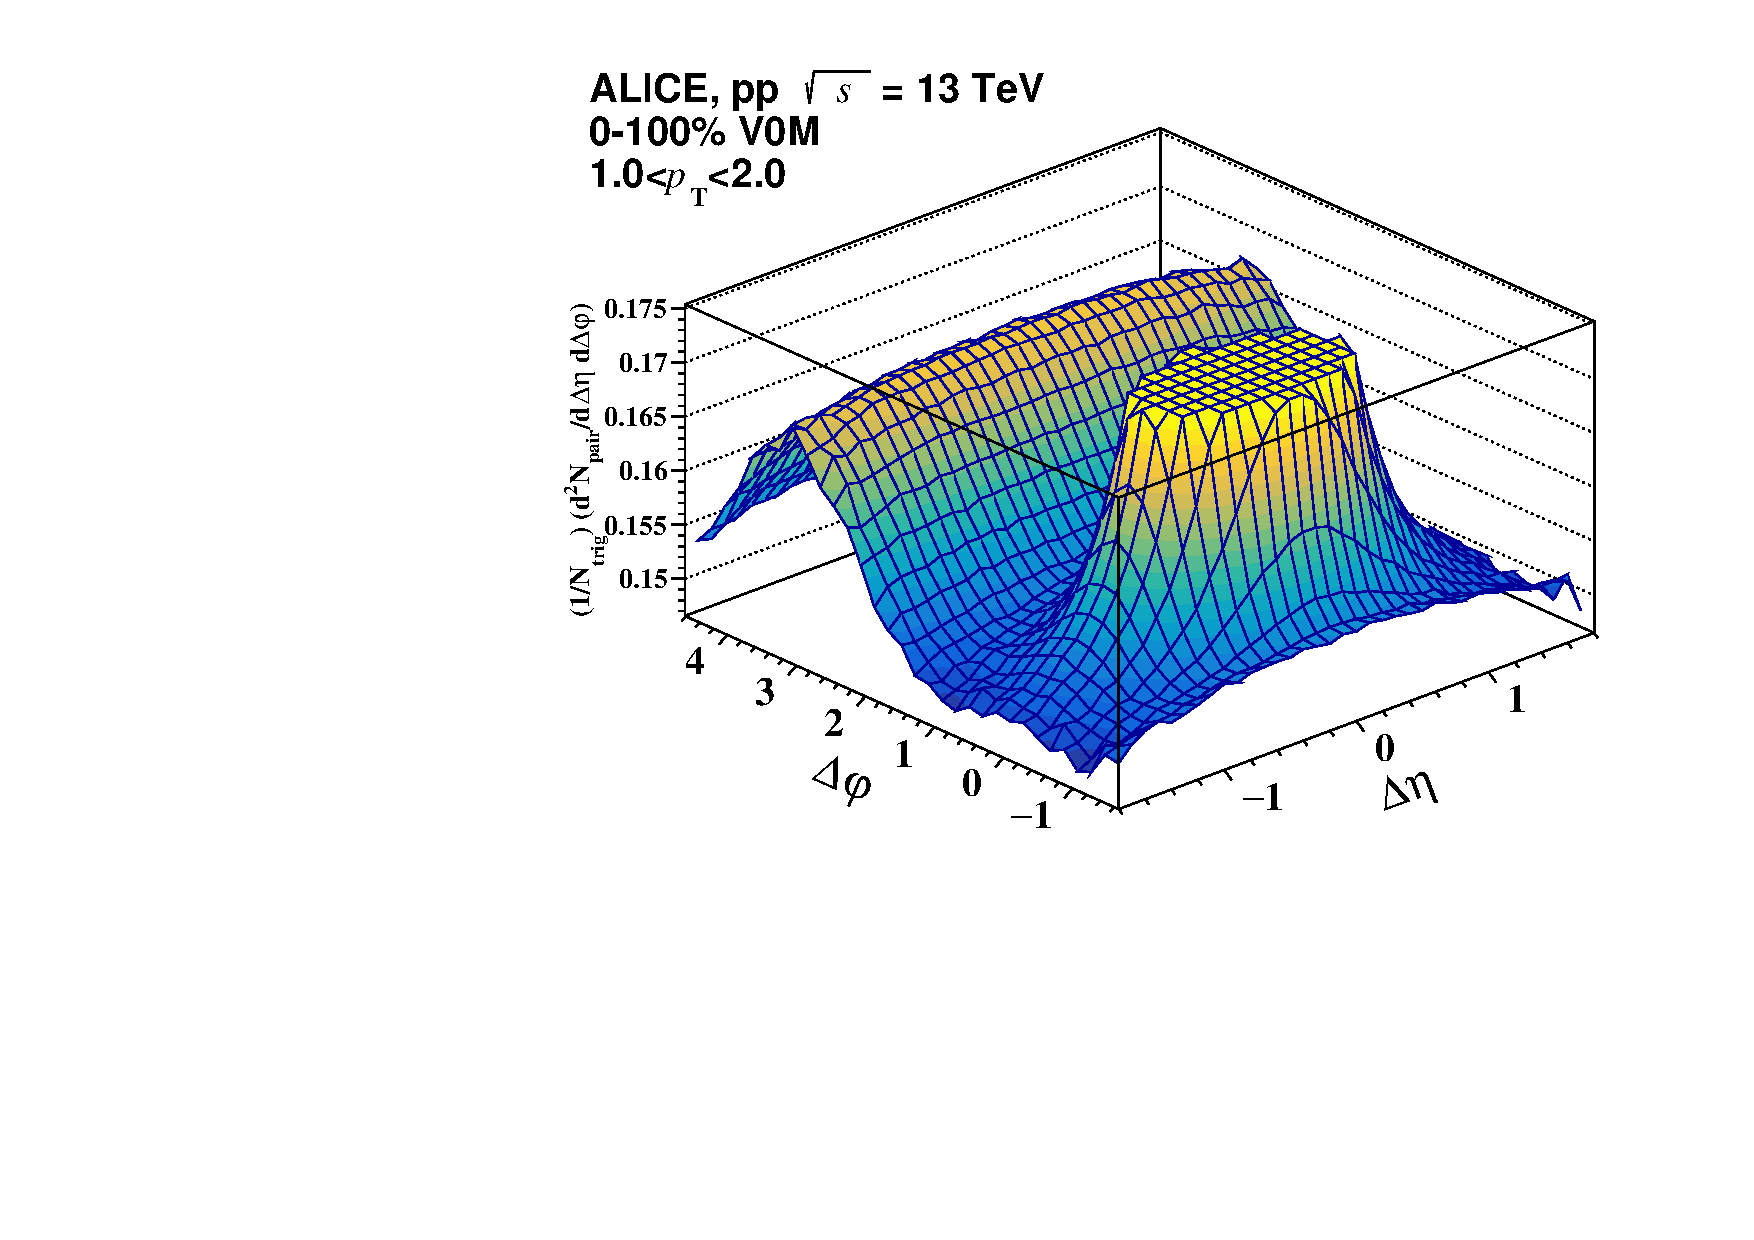
\includegraphics[width=0.47 \textwidth]{./figures/corrmb.pdf} }
	\caption{ Dihadron correlation functions as functions of $\Delta\eta$ and $\Delta\varphi$ in high-multiplicity (0--0.1\%, left) and minimum-bias events (0--100\%, right). The intervals of $\pttrig$ and $\ptassoc$ are equally $1 < \it{p}_{\rm{T}} < $2 GeV/$c$. }
	\label{fig:PlotCorrMBHMT}
\end{figure}

Figure~\ref{fig:PlotCorrMBHMT} shows the per-trigger yield obtained from Eq. 1 for $1 < \pttrig~\mathrm (\ptassoc) < $2 GeV/$c$ in pp collisions at $\sqrt{\it{s}} = $\unit{13} {\rm{}TeV} for high-multiplicity (left) and minimum bias events (right panel). The ridge structure is clearly observed in the high-multiplicity class while it is less visible and conclusive in the minimum bias events. The away-side yield is populated mostly by back-to-back jet correlations.

\begin{figure}[h!]
	\centering
	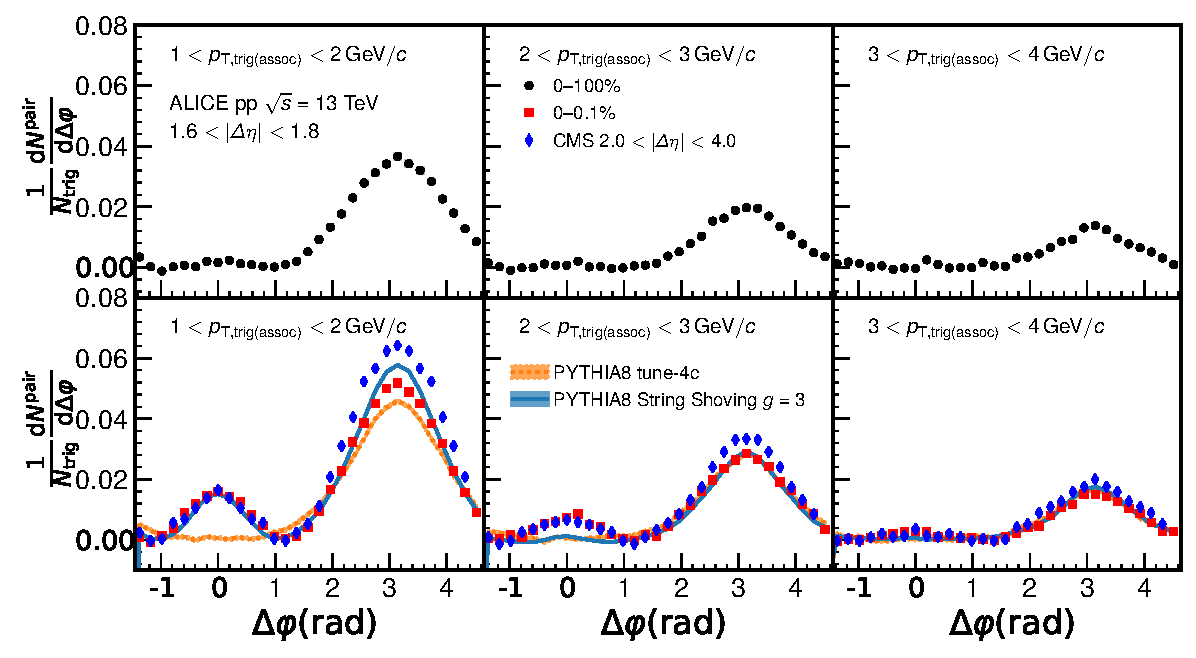
\includegraphics[width=0.9\linewidth]{./figures/Fig2_PlotDeltaPhi.pdf}
	\caption{One-dimensional $\Delta\varphi$ distribution in the large $\Delta\eta$ projection for three transverse momentum intervals in high-multiplicity (lower panels) and minimum bias (upper panels) events after ZYAM subtraction. Transverse momentum ranges of trigger particles and associated particles are $1<\pt<$2 (left), 2$<\pt<$3 (middle) and 3$<\pt<$4 GeV/$c$ (right), respectively. The presented model predictions were calculated using $\pythiashoving$, $\pythiam$, and $\epos$.}
	\label{fig:PlotDeltaPhi}
\end{figure}
 
Figure~\ref{fig:PlotDeltaPhi} shows Delta phi projections of the two-particle correlation functions obtained in the range 1.6$<|\Delta \eta |<$1.8 for several track $\pt$ intervals after ZYAM subtraction, see Eq. 2. Results are shown for various $\it{p}_{\rm{T}}$ intervals in the minimum bias class (upper) and the high-multiplicity class (lower) down to 1 GeV/$c$ where non-flow contamination is negligible. The near-side ($\Delta\varphi\sim 0$) ridge in the high-multiplicity class is clearly observed in all transverse momentum ranges studied while there is no hint of the signal in the minimum bias class. Within the range of analyzed particle $\pt$, yield in the near-side ridge decreases with increasing $\pt$ in the high-multiplicity class. The measurements in the high-multiplicity class are compared to the results published by the CMS collaboration~\cite{Khachatryan:2015lva}. In case of the CMS measurement, charged particle multiplicity was obtained by counting $\pt>0.4$ GeV/$c$ tracks in $|\eta|<$2.4. In our analysis, event multiplicity is determined from the forward V0 detectors. The difference in multiplicity selection between ALICE (forward) and CMS (mid-rapidity) was studied using PYTHIA 8 simulations and it was found that the CMS multiplicity is ${\approx}20\,\%$ larger than the ALICE one when compared in the acceptance region of the measurements reported here, $|\eta|<$0.9. Near-side ridges in all transverse momentum ranges are comparable to each other within the uncertainties. The larger away-side yields observed in \cite{Khachatryan:2015lva} can be attributed to the difference in $\eta$ acceptance for the multiplicity selection, which overlaps somewhat with the $\eta$ region in Fig.~\ref{fig:PlotDeltaPhi} for CMS results. The ALICE data are compared with model predictions where we apply a comparable high-multiplicity selection and $\Delta\eta$ projection range. Selection of high-multiplicity events in models was done by requiring a minimal number of charged particles that pass the V0M acceptance. This threshold was set to 105, which was tuned to reach the top 0-0.1\% centrality selection using $\pythiam$. The threshold for $\epos$ or $\pythiashoving$ is 110 or 108, respectively. The $\pythiashoving$ gives good estimates of the near-side ridge yield and slightly overestimates the away-side yield for the interval of 1$<\it{p}_{\rm{T}}<$2 GeV/$c$. However, the $\pythiashoving$ underestimates the near-side ridge yield for $\it{p}_{\rm{T}}>$2 GeV/$c$. $\pythiam$ does not show any near-side ridge as expected. It slightly underestimates the away-side peak for $1<\it{p}_{\rm{T}}<$2 GeV/$c$ and gives good estimates for $\it{p}_{\rm{T}}>$2 GeV/$c$. On the other hand, $\epos$ describes quantitatively better the $\pt$ dependence in the 2$<\it{p}_{\rm{T}}<$4 GeV/$c$ range, while overestimating the near-side ridge yield for the $\it{p}_{\rm{T}}<$2 GeV/$c$ range. 


\begin{figure}[h!]
	\centering
	\subfigure{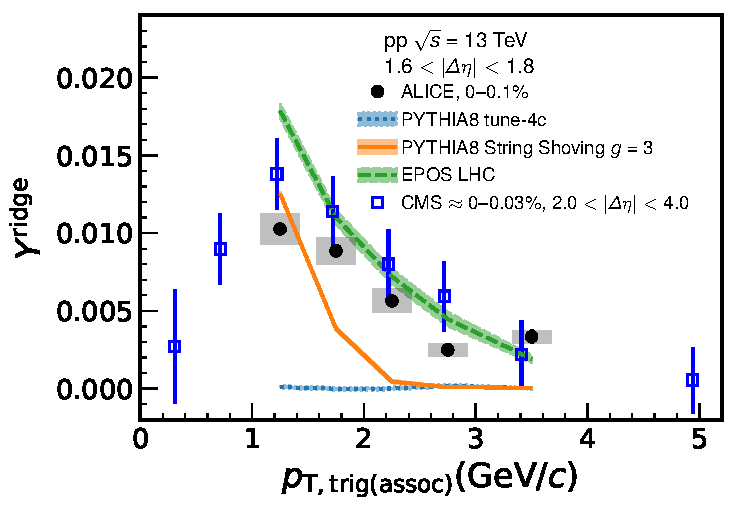
\includegraphics[width=0.99\textwidth]{./figures/Fig3_PlotRidgeYield.pdf}}
	\caption{ Fully corrected near-side ridge yield as a function transverse momentum. The filled circles denote the measurement with ALICE. The CMS measurement~\cite{Khachatryan:2015lva} is represented by open blue box markers and extends down to lower $\pt$ due to the larger $\Delta\eta$ acceptance. The three lines show model predictions from $\pythiam$ (blue line), $\pythiashoving$ (orange line) and $\epos$ (green line).}
	\label{fig:PlotYSpect}
\end{figure}

Figure~\ref{fig:PlotYSpect} shows the near-side ridge yield measured in high-multiplicity events as a function of transverse momentum. The ALICE data are with results from CMS~\cite{Khachatryan:2015lva}.
%The ridge yields as a function of the transverse momentum are shown in Fig.~\ref{fig:PlotYSpect} in the high-multiplicity class and compared to \cite{Khachatryan:2015lva}.
Taking into account the differences in acceptance of both measurements and chosen multiplicity estimator, the slight disagreement between the two sets of results could be expected. The data is also compared with model calculations. $\pythiam$ gives zero ridge yields since it does not account for the ridge effect. $\pythiashoving$ describes the yield qualitatively. however the predicted yield decreases more rapidly than the measured one as $\pttrigassoc$ increases. $\epos$, unlike $\pythiashoving$, describes well the $\pt$ dependence of the ridge yield for the $\it{p}_{\rm{T}}>$2 GeV/$c$ range, while predicting larger yield for $\it{p}_{\rm{T}}<$2 GeV/$c$.

\subsection{Event-scale dependence of the ridge yield}
\begin{figure}[h!]
	\centering
	\subfigure{ 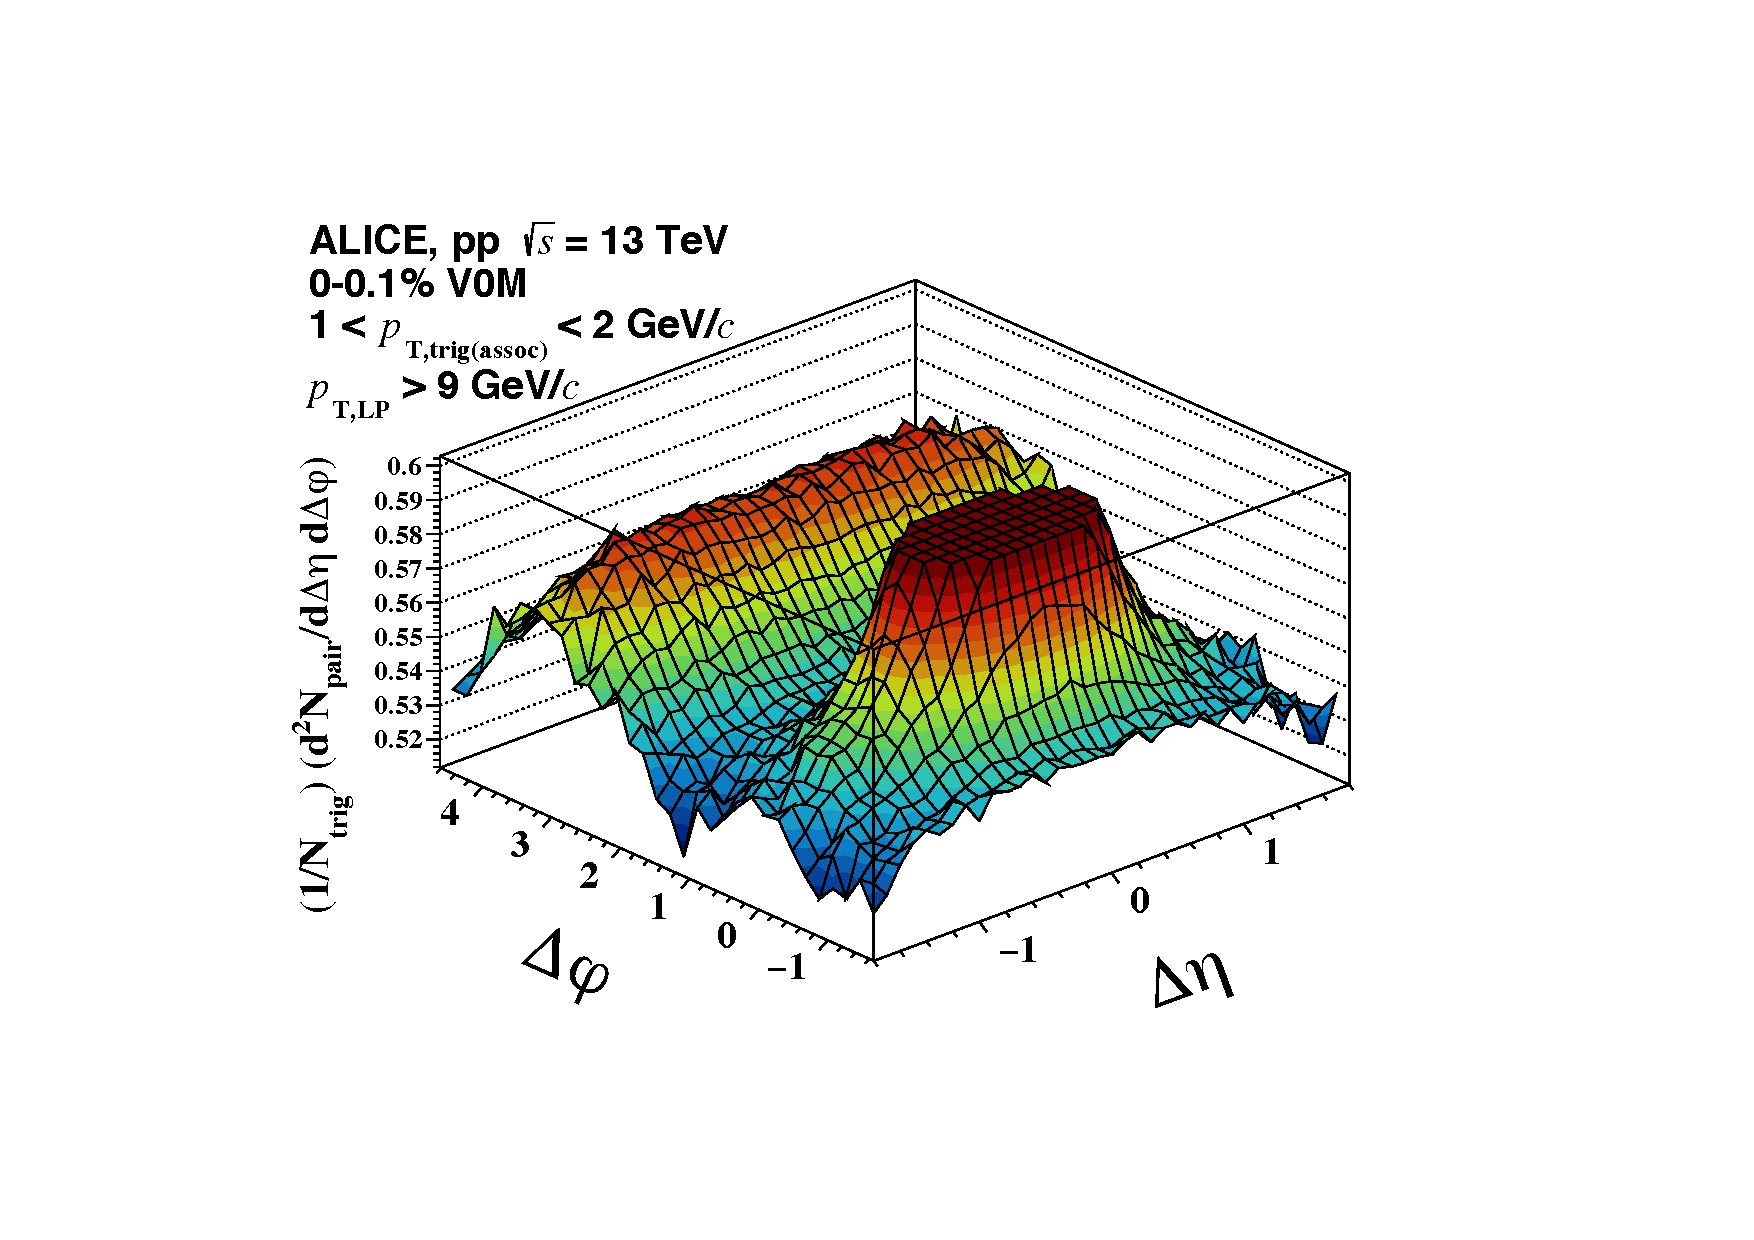
\includegraphics[width=0.47 \textwidth]{./figures/corrlh.pdf} }
	\subfigure{ 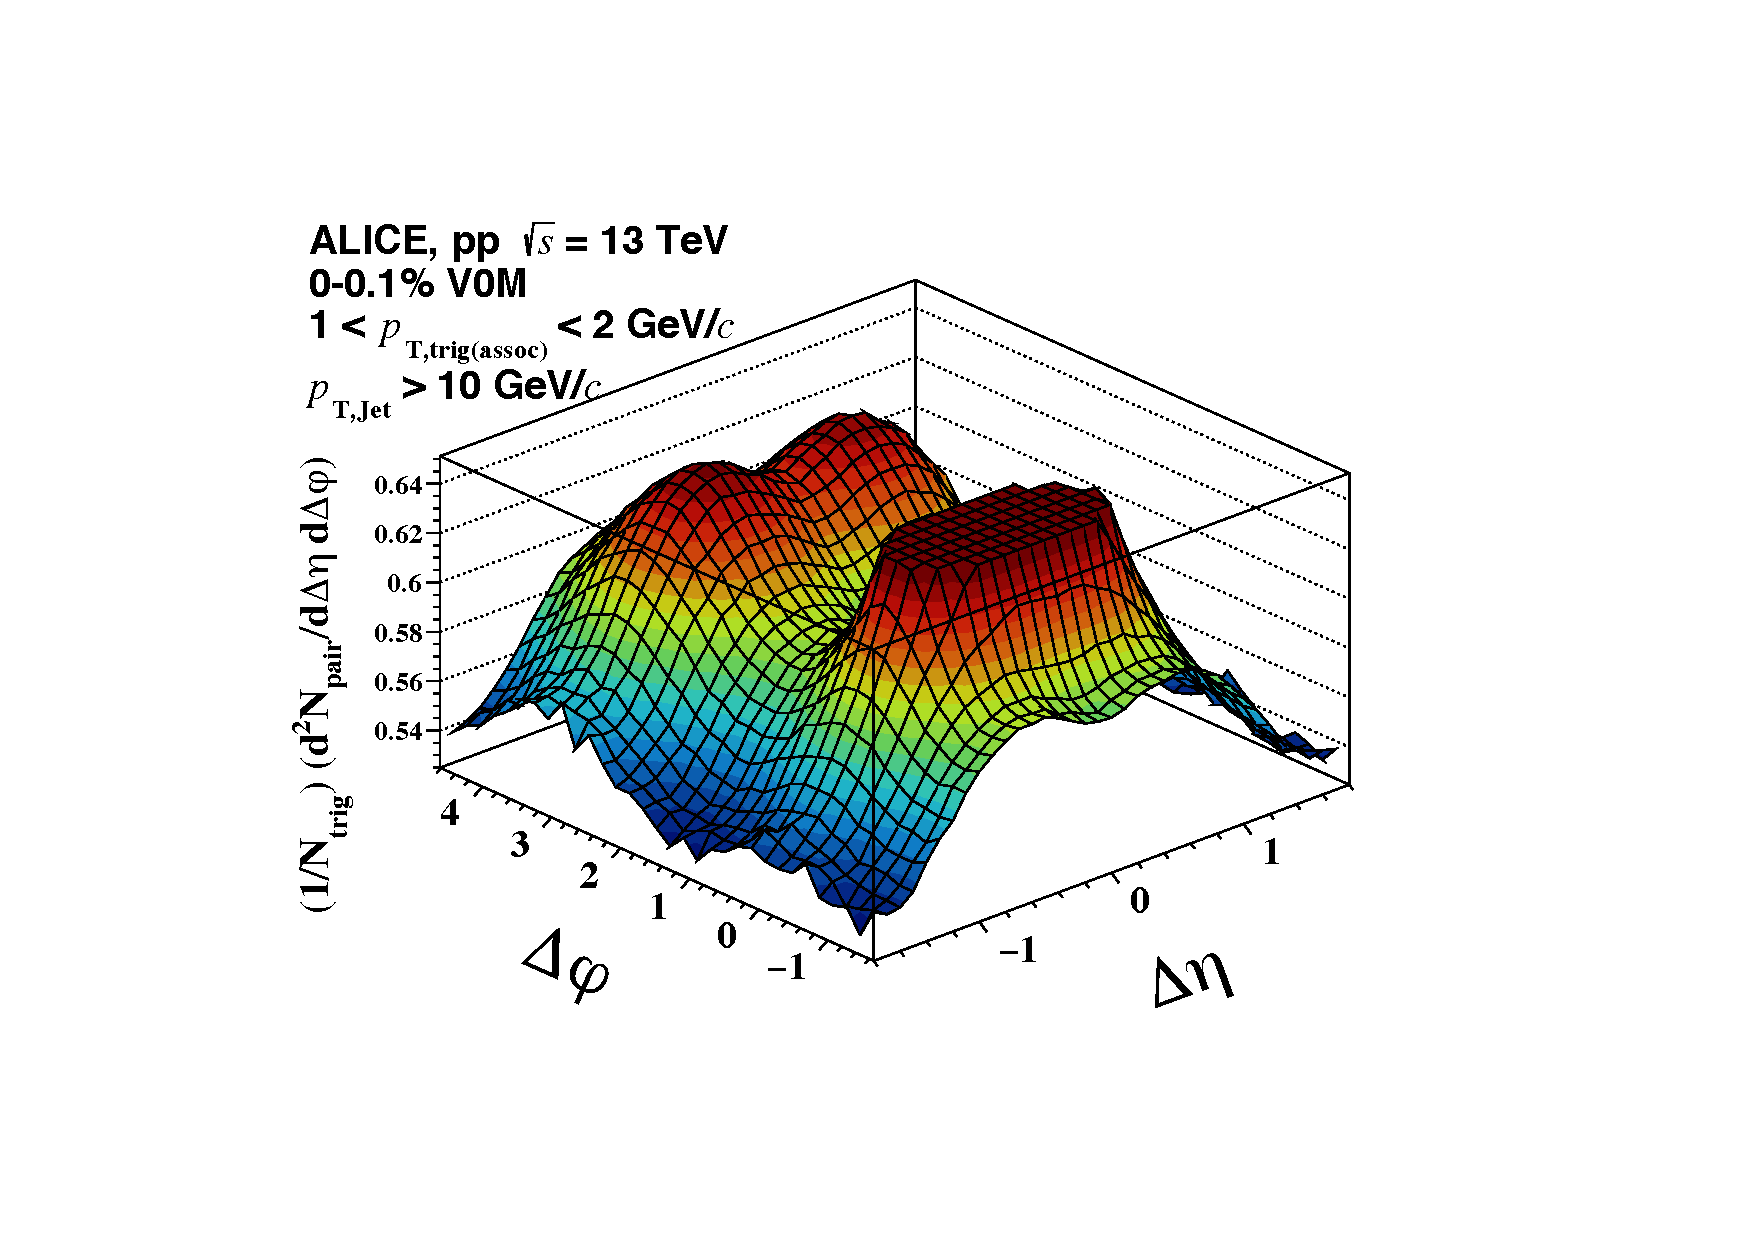
\includegraphics[width=0.47 \textwidth]{./figures/corrjet.pdf} }
	\caption{ Two-dimensional correlation functions as a function of $\Delta\eta$ and $\Delta\varphi$ in high-multiplicity events where a selection on event-scale was required in addition. The interval of $\pttrig$ and $\ptassoc$ is 1$<\pt<$2 GeV/$c$. Left: HM events with a $\ptlead>$ 9 GeV/$c$ leading track. Right: HM events with a $\ptjet>$ 10 GeV/$c$.}
	\label{fig:PlotCorrHMTSel}
\end{figure}

The ridge yield is further studied with respect to two different event-scales. In the first measurement, the event-scale is set by requiring a minimum $\pt$ cutoff on a leading track in event (denoted as $\ptlead$), while in the second measurement, we impose a minimum $\pt$ cutoff on a leading jet (denoted as $\ptjet$). As shown in Fig.~\ref{fig:PlotCorrHMTSel}, the ridge structure for $1< \pttrig\,(\ptassoc) <2$ GeV/$c$ still persists in high-multiplicity pp collisions with $\ptlead>9$~GeV/$c$ (left) and $\ptjet>10$~GeV/$c$ (right).  %The interval is the same to the measured ridge yield is maximum without the event-scale selection.
It is worth noting that the correlation function obtained with the minimum $\ptjet$ selection has a double peak structure which is oriented along the $\Delta\eta$ axis at $\Delta\varphi=\pi$. This structure emerges due to the restricted acceptance of jet tagging, $|\eta_{\rm{jet}}|<$0.4.

\begin{figure}[h!]
	\centering
	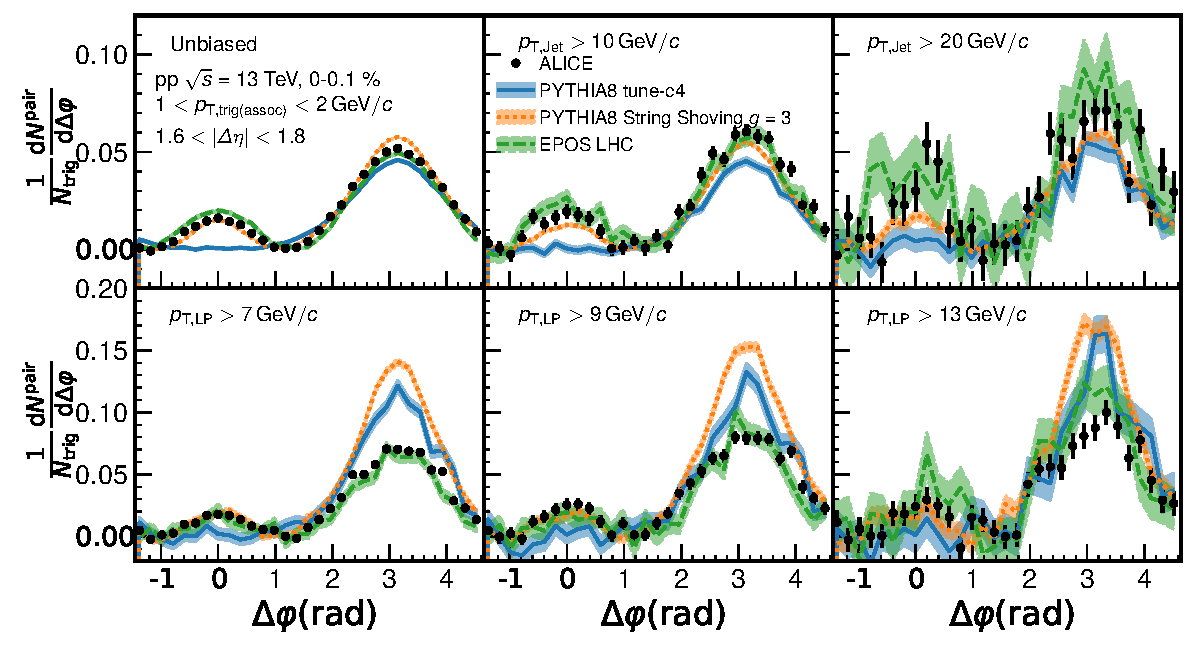
\includegraphics[width=0.99\linewidth]{./figures/Fig5_PlotDeltaPhiESE.pdf}
	\caption{ $\Delta\varphi$ projections of the correlation functions constrained to 1.6$<|\Delta\eta|<$1.8 in HM events with an additional event-scale bias. Top: with an imposed cut on leading jet $\pt$,  bottom: with an imposed cut on leading hadron $\pt$. ALICE data are compared with prediction of models.}
	\label{fig:PlotDeltaPhiESE}
\end{figure}

Figure~\ref{fig:PlotDeltaPhiESE} shows projected $\Delta\varphi$ distributions of the correlation functions in $1.6<|\Delta\eta|<1.8$ with the minimum $\ptlead$ (lower) and $\ptjet$ (upper) requirement. Even with the event-scale selection, the ridge is still visible at the near-side. The near-side ridge peak increases as the thresholds of $\ptlead$ and $\ptjet$ increase compared to the one measured in unbiased events. The results are compared with $\pythiashoving$, $\pythiam$, and $\epos$ calculations. Near-side ridge peaks are qualitatively reproduced by $\pythiashoving$ and $\epos$. On the other hand, $\pythiam$ does not show the  near-side ridge peak for neither of the two event-scale selections, but it gives compatible results for the away-side yield as $\pythiashoving$.
%Both models describe the away-side yield with the $\ptjet$ selection and overestimate away-side yield with the $\ptlead$ selection.

\begin{figure}[h!]
	\centering
	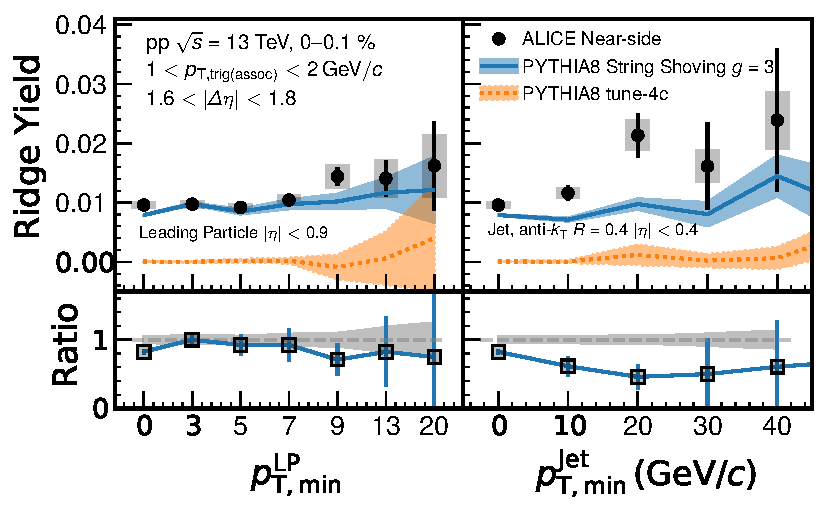
\includegraphics[width=0.89\linewidth]{./figures/Fig6_RidgeYieldESE.pdf}
	\caption{Near-side ridge yield as a function of the $\ptlead$ (left) and $\ptjet$ (right) bias. Data points (filled circles) show the ALICE measurement. They are compared to predictions of models which are represented by color bands. The bottom panel shows a ratio of the models to the data. The uncertainty on the data is represented by the gray band centered around unity.}
	\label{fig:RidgeYield_ESE}
\end{figure}

The ridge yields as functions of the minimum $\ptlead$ ($\it{p}^{\rm{LP}}_{\rm{T,min}}$) and $\ptjet$ ($\it{p}^{\rm{Jet}}_{\rm{T,min}}$) selections are shown in Fig.~\ref{fig:RidgeYield_ESE}. High-multiplicity events with imposed event-scale bias exhibit increased ridge yields when compared to unbiased HM events. A moderate increase of the ridge yields as a function of $\ptlead$ or $\ptjet$ is observed and there is no difference between the two event selections within the uncertainties.
Comparison to model calculations suggests that $\pythiashoving$ gives comparable trend with data, but underestimates the ridge yield. On the other hand, $\epos$, which also provides a trend comparable with the data, overestimates the ridge yield. The origin of the enhanced ridge yields for higher momentum jet-tagged events is not clear to date but it might be related with the expected shorter impact parameters for dijet or multi-jet production events studied in~\cite{Frankfurt:2010ea}.

\begin{figure}[h!]
	\centering
	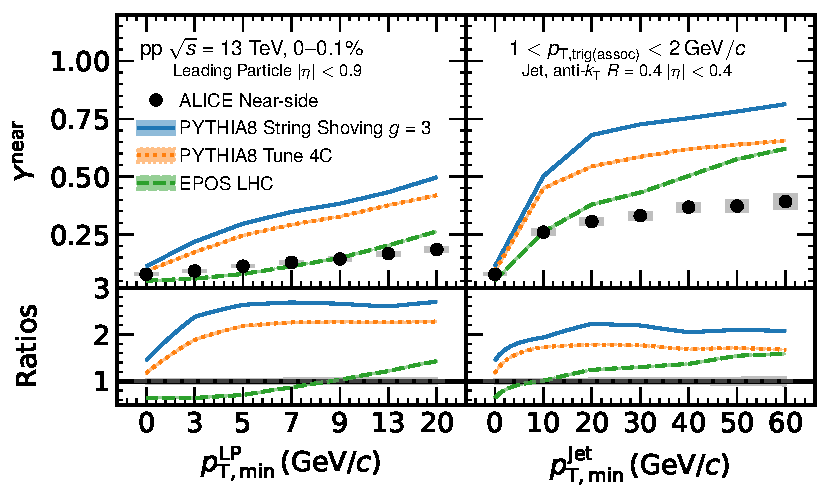
\includegraphics[width=0.89\linewidth]{./figures/Fig9_JetYieldESE.pdf}
	\caption{ Near-side jet-like peak yield with respect to the minimum leading particle (left) and jet selections (right). The filled circles show measurement with ALICE. The measurements are compared with model descriptions from $\pythiam$, $\pythiashoving$, and $\epos$ for both selections.}
	\label{fig:JetYield_ESE}
\end{figure}

Finally, near-side jet-like peak yield was measured as a function of minimum $\ptlead$ and $\ptjet$ threshold in Fig.~\ref{fig:JetYield_ESE} to further test the models that aim to describe the near-side ridge.
%quantify the trend of the jet yield.
$\epos$ provides comparable estimates of the near-side jet-like peak yield, while $\pythiam$ and $\pythiashoving$ overestimate near-side yields for both selections.

In all models where the ridge is due to final-state interactions, e.g., $\epos$ and PYTHIA 8 String Shoving, one also expects the near-side jet-like peak yield to be affected. This can be observed when comparing the measured near-side jet yields with PYTHIA 8 calculations with and without String Shoving. The new ALICE results therefore provide constraints beyond traditional ridge measurements that challenge existing models.